\documentclass{standalone}
\usepackage{pgfplots}
\usepackage{lmodern}
\pgfplotsset{compat=1.17}

\begin{document}

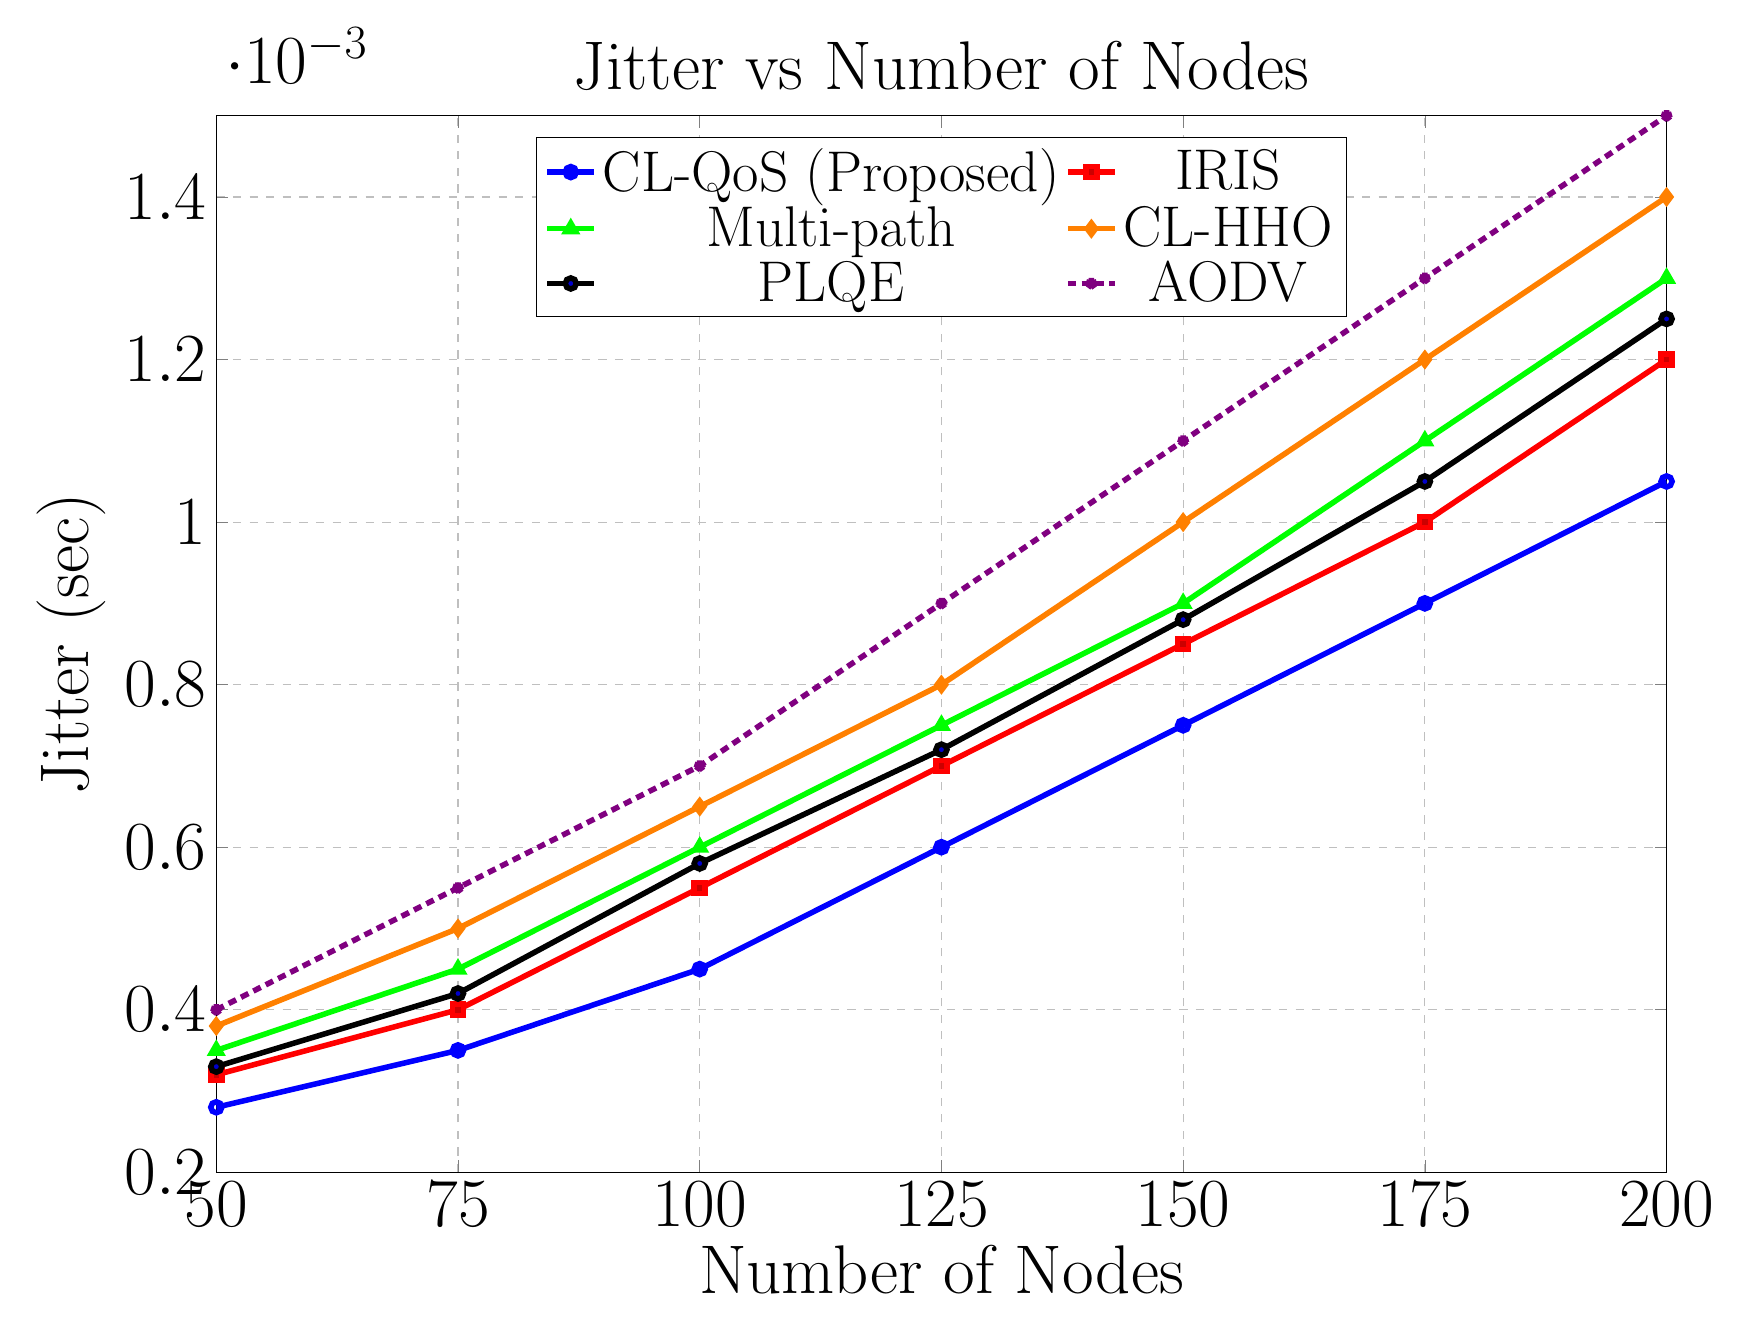
\begin{tikzpicture}
\begin{axis}[
    width=20cm,
    height=15cm,
    tick label style={font=\fontsize{24}{28}\selectfont},
    label style={font=\fontsize{24}{28}\selectfont},
    title style={font=\fontsize{24}{28}\selectfont},
    title={Jitter vs Number of Nodes},
    xlabel={Number of Nodes},
    ylabel={Jitter (sec)},
    xmin=50, xmax=200,
    ymin=0.0002, ymax=0.0015,
    xtick={50,75,100,125,150,175,200},
    ytick={0.0002,0.0004,0.0006,0.0008,0.0010,0.0012,0.0014},
    legend columns=2,
    legend style={
        font=\fontsize{22}{26}\selectfont,
        at={(0.5,0.98)},
        anchor=north,
        draw=black,
        fill=white
    },
    grid=both,
    grid style=dashed
]

% CL-QoS (REAL DATA - SMOOTHED)
\addplot+[mark=o,color=blue,line width=2pt] coordinates {
    (50,0.00028)(75,0.00035)(100,0.00045)(125,0.00060)
    (150,0.00075)(175,0.00090)(200,0.00105)
};

% IRIS
\addplot+[mark=square*,color=red,line width=2pt] coordinates {
    (50,0.00032)(75,0.00040)(100,0.00055)(125,0.00070)
    (150,0.00085)(175,0.0010)(200,0.0012)
};

% Multi-path
\addplot+[mark=triangle*,color=green,line width=2pt] coordinates {
    (50,0.00035)(75,0.00045)(100,0.00060)(125,0.00075)
    (150,0.00090)(175,0.0011)(200,0.0013)
};

% CL-HHO
\addplot+[mark=diamond*,color=orange,line width=2pt] coordinates {
    (50,0.00038)(75,0.00050)(100,0.00065)(125,0.00080)
    (150,0.0010)(175,0.0012)(200,0.0014)
};

% PLQE
\addplot+[mark=*,color=black,line width=2pt] coordinates {
    (50,0.00033)(75,0.00042)(100,0.00058)(125,0.00072)
    (150,0.00088)(175,0.00105)(200,0.00125)
};

% AODV
\addplot+[mark=star,color=violet,line width=2pt] coordinates {
    (50,0.00040)(75,0.00055)(100,0.00070)(125,0.00090)
    (150,0.0011)(175,0.0013)(200,0.0015)
};

\legend{CL-QoS (Proposed), IRIS, Multi-path, CL-HHO, PLQE, AODV}

\end{axis}
\end{tikzpicture}

\end{document}